\bb[itemsep=5pt]
\ii Consider the differential equation 
\[
f''(x)+f'(x)=x^2+x+1 \tag{$*$}
\]

The theory of ODE's tells us that there are infinitely many solutions $f(x)$ to $(*)$. We will use linear algebra to find infinitely many polynomial solutions. 
\bb
\ii First define $T\colon P_{3}\rightarrow P_{2}$ as $T(f)=f''(x)+f'(x)$. Explain why $T(f)$ indeed lies in $P_2$ and show that $T$ is linear. 
\ii Compute $A=[T]_{B}^{B'}$ where $B$ and  $B'$ are the standard bases of $P_{3}$ and $P_{2}$, respectively. 
\ii Determine $\NS(A)$ and $\CS(A)$. 
\ii Find all solutions in $P_3$ to the differential equation $(*)$. (First solve the relevant matrix equation involving $A$, then ``lift up" to $P_3$. )
\ee
{\footnotesize Note: though we have found all {\em polynomial solutions} to the differential equation $(*)$, we have not found {\em all} solutions. Observe that $g(x)=e^{-x}$ is a solution to the corresponding homogeneous equation $f''+f'=0$, It follows from basic ODE theory that we can add $ce^{-x}$ to any of our solutions in (d) to get a new solution. Our analysis didn't catch these solutions as we restricted our attention to $P_3$. }
\\
\begin{solution}
\ \\(a) The usual proof shows $T$ is linear. Since taking the derivative knocks down the degree of a polynomial by 1, it's clear that if $p(x)$ has degree at most $3$, then $T(p)=p''+p'$ will have degree at most $2$.

(b) Let $B=\{1,x,x^2,x^3\}$ and $B'=\{1, x, x^2\}$. The usual recipe for $[T]_{B',B}$ begins by computing 
\[
T(1)=0, T(x)=1, T(x^2)=2+2x, T(x^3)=6x+3x^2.
\] 
Taking coordinate vectors with respect to $B$ and placing these in columns yields 
\[
A=\begin{bmatrix}
0&1&2&0\\
0&0&2&6\\
0&0&0&3
\end{bmatrix}.
\]
(c) The rank of $A$ is clearly 3 (look at rows), and by inspection we see that $\{(1,0,0), (2,2,0), (0,6,3)\}$ is a basis for $\CS(A)$. Since $\dim\CS(A)=3$ and $\CS(A)\subset\R^3$, it follows from the Subspace Dimension Theorem that $\CS(A)=\R^3$.

Since $\rank(A)=3$, it follows from R-N that $\nullity(A)=4-3=1$. To come up with a basis for $\NS(A)$ we simply need to find one nonzero element of $\NS(A)$. We see $\{(1,0,0)\}$ does the trick. 

What does all this mean about $T$? Since $\CS(A)=\R^3$, it follows that $\range(T)=P_2$. Thus for {\em any} $q(x)\in P_2$, we can find a $p(x)\in P_3$ with $T(p)=p''(x)+p'(x)=q(x)$. This means not only can we solve the given differential equation, we can solve any similar equation of the form $f''+f'=q$, where $q$ is a polynomial in $P_2$.  

Furthermore, as we will see, the fact that $\NS(A)$ is nontrivial will mean that we can always find infinitely many solutions to $(*)$. 

(d) The polynomial $x^2+x+1$ corresponds via $[\hspace{8pt}]_{B'}$ to the vector $\begin{bmatrix}1\\ 1\\ 1\end{bmatrix}$. All solutions $\boldx$ to
\[
A\boldx=\begin{bmatrix}1\\ 1\\ 1\end{bmatrix}
\] 
will lift up to the solutions $p$ to $T(p)=x^2+x+1$. 

Using GE, we see the general solution to the matrix equation is 
\[
\boldx=c\begin{bmatrix}1 \\ 0 \\ 0 \end{bmatrix}+\begin{bmatrix}1\\-\frac{1}{2}\\ \frac{1}{3} \end{bmatrix}
\]
Thus the general {\em polynomial} solution to the original differential equation is 
\[
p(x)=c+(1-\frac{1}{2}x^2+\frac{1}{3}x^3)=(c+1)-\frac{1}{2}x^2+\frac{1}{3}x^3.
\]

\end{solution}
\ii Define $T\colon M_{22}\rightarrow M_{22}$ by $T(A)=A^T-A$. 
\bb
\ii Compute $A=[T]_B$ where $B$ is the standard basis for $M_{22}$. 
\ii Compute bases for $\NS(A)$ and $\CS(A)$.
\ii Use your result in (b) to give bases for $\NS(T)$ and $\range(T)$. 
\ii Identify $\NS(T)$ and $\range(T)$ as familiar subspaces of matrices. 
\ee
\begin{solution}
\ \\
(a) The usual recipe yields 
\[
A=\begin{bmatrix}[rrrr]0&0&0&0\\
0&-1&1&0\\
0&1&-1&0\\
0&0&0&0
\end{bmatrix}.
\]
We have $\NS(A)=\Span(\{(1,0,0,0), (0,0,0,1), (0,1,1,0)\}$ and $\CS(A)=\Span(\{(0,-1,1,0)\}$. 

By lifting we get that 
\[
\NS(T)=\Span\left(\left\{\begin{bmatrix}[rr] 1&0\\ 0&0\end{bmatrix}, \begin{bmatrix}[rr] 0&0\\ 0&1\end{bmatrix}, \begin{bmatrix}[rr]0&1\\ 1&0 \end{bmatrix}\right\}\right), \ \range(T)=\Span\left(\left\{\begin{bmatrix}[rr] 0&-1\\ 1&0\end{bmatrix}\right\}\right).
\]
From these descriptions it follows easily that $\NS(T)$ is the subspace of all symmetric matrices, and $\range(T)$ is the subspace of all skew-symmetric matrices. 
\end{solution}
\ii Let $T_{\alpha}\colon\R^2\rightarrow\R^2$ be reflection through the line $\ell_{\alpha}$, as defined previously in Exercise \ref{Ex:refl} in Section 5.1-5.2. Recall also that $T_{\alpha}$ is an origin-fixing isometry, hence a linear transformation. 
\\
Compute the matrix $A$ such that $T_{\alpha}=T_A$ as follows: first compute $A'=[T_{\alpha}]_{B'}$ where $B'=\{\boldv_1,\boldv_2\}$ is a basis for $\R^2$ satisfying $\boldv_1\in \ell_\alpha$, $\boldv_2\in \ell_\alpha^\perp$; then compute $A=[T_{\alpha}]_B$ from $A'$ using the change of basis formula for transformations. 
\\
Note: your vectors $\boldv_1, \boldv_2$ will be expressed in terms of $\alpha$ (and some trig functions). 
\\
Check that you get the same answer from before! 
\\
\begin{solution} 
%\ \\
\noindent 
Since $B$ is the standard basis, it turns out that The matrix $A=[T]_B$ is just the matrix that defines the given linear transformation. We computed this in an earlier exercise. We got
\[
A=\begin{bmatrix}[rr]
\cos(2\alpha)&\sin(2\alpha)\\
\sin(2\alpha)&-\cos(2\alpha)
\end{bmatrix}=\begin{bmatrix}[rr]
-1/2&\sqrt{3}/2\\
\sqrt{3}/2&1/2
\end{bmatrix}.
\]
Given a basis as specified, the matrix $A'=[T]_{B'}$ is simpler because the action of $T$ on this basis is simpler: $T(\boldv_1)=\boldv_1$ and $T(\boldv_2)=-\boldv_2$ (draw a picture!). Thus 
\[
A'=\begin{bmatrix}
\vert&\vert\\
[T(\boldv_1)]_{B'}&[T(\boldv_2)]_{B'}\\
\vert&\vert
\end{bmatrix}
=\begin{bmatrix}
\vert&\vert\\
[\boldv_1]_{B'}&[-\boldv_2]_{B'}\\
\vert&\vert
\end{bmatrix}=
\begin{bmatrix}[rr]
1&0\\
0&-1
\end{bmatrix}.
\]
Let's actually pin down a basis $B'$ as specified. The basis elements are necessarily orthogonal (from the description); I will make them orthonormal to make my life as easy as possible!  The vector $\boldv_1$ points along $\ell_{\alpha}$: a unit vector fitting this description is $\boldv_1=(\cos(\alpha), \sin(\alpha))$. The vector $\boldv_2$ should be a unit vector orthogonal to $\boldv_1$: I pick $\boldv_2=(-\sin(\alpha), \cos(\alpha))$. 

We need to compute change of bases matrices between $B'$ and the standard basis $B$. Again we find ourselves in the special setting where $\underset{B'\rightarrow B}{P}$ is built by simply putting the elements of $B'$ as its columns. Thus we have 
\begin{align*}
\underset{B'\rightarrow B}{P}&=\begin{bmatrix}
[rr]
\cos(\alpha) &-\sin(\alpha)\\
\sin(\alpha)&\cos(\alpha)
\end{bmatrix}\\
\\
\underset{B\rightarrow B'}{P}&=(\underset{B'\rightarrow B}{P})^{-1}\\
&=(\underset{B'\rightarrow B}{P})^{T} &\text{(since columns of $\underset{B'\rightarrow B}{P}$ are orthonormal!}\\
&=\begin{bmatrix}
[rr]
\cos(\alpha) &\sin(\alpha)\\
-\sin(\alpha)&\cos(\alpha)
\end{bmatrix}
\end{align*}
Lastly, we compute 
\begin{align*}
A=[T]_B&=(\underset{B\rightarrow B'}{P})^{-1}[T]_{B'}\underset{B\rightarrow B'}{P}\\
&=\underset{B'\rightarrow B}{P}[T]_{B'}\underset{B\rightarrow B'}{P}\\
&=\begin{bmatrix}
[rr]
\cos(\alpha) &-\sin(\alpha)\\
\sin(\alpha)&\cos(\alpha)
\end{bmatrix}
\begin{bmatrix}[rr]
1&0\\
0&-1
\end{bmatrix}
\begin{bmatrix}
[rr]
\cos(\alpha) &\sin(\alpha)\\
-\sin(\alpha)&\cos(\alpha)
\end{bmatrix}\\
&=
\begin{bmatrix}
\cos^2(\alpha)-\sin^2(\alpha) & 2\sin(\alpha)\cos(\alpha)\\
2\sin(\alpha)\cos(\alpha)&\sin^2(\alpha)-\cos^2(\alpha)
\end{bmatrix}
\\
&=\begin{bmatrix}[rr]
\cos(2\alpha)&\sin(2\alpha)\\
\sin(2\alpha)&-\cos(2\alpha)
\end{bmatrix}. \ \checkmark
\end{align*}
\end{solution}
\ii Let $T:P_2\rightarrow P_3$ be the linear transformation defined by $T(p)=x\cdot p(x-3)$. Find $[T]_{B}^{B'}$ relative to the bases $B=\{1,x,x^2\}$ and $B' = \{1,x,x^2,x^3\}$.
\\
\begin{solution}
\noindent By the formula for $T$
\begin{eqnarray*}
T(1) &=& x(1) = x\\
T(x) &=& x(x-3) = x^2 - 3x\\
T(x^2) &=& x^3-6x^2+9x
\end{eqnarray*}
Taking these vectors relative the the basis $B'$, we can write
$$
[T]_{B}^{B'} = 
\begin{bmatrix}[ccc]
0&0&0\\
1&-3&9\\
0&1&-6\\
0&0&1
\end{bmatrix}
$$
\end{solution}
\ii Let $T:P_2 \rightarrow M_{22}$ be the linear transformation defined by
$$
T(p) =
\begin{bmatrix}[cc]
p(0)&p(1)\\
p(-1)&p(0)
\end{bmatrix}
$$
let $B$ be the standard basis for $M_{22}$, let $B'=\{1,x,x^2\}$ and $B''=\{1,1+x,1+x^2\}$ be bases for $P_2$. Find $[T]_{B'}^{B}$ and $[T]_{B''}^{B}$.
\\
\begin{solution}
\noindent Lets work on $[T]_{B}^{B'}$ first. By the formula for $T$
\begin{eqnarray*}
T(1) &=&
\begin{bmatrix}[rr]
1&1\\
1&1
\end{bmatrix}\\
T(x) &=&
\begin{bmatrix}[rr]
0&1\\
-1&0
\end{bmatrix}\\
T(x^2) &=&
\begin{bmatrix}[rr]
0&1\\
1&0
\end{bmatrix}\\
\end{eqnarray*}
Taking these vectors relative the the basis $B$, we can write
$$
[T]_{B}^{B'} =
\begin{bmatrix}[rrr]
1&0&0\\
1&1&1\\
1&-1&1\\
1&0&0
\end{bmatrix}
$$
Now for $[T]_{B}^{B''}$. By the formula for $T$
\begin{eqnarray*}
T(1) &=&
\begin{bmatrix}[rr]
1&1\\
1&1
\end{bmatrix}\\
T(1+x) &=&
\begin{bmatrix}[rr]
1&2\\
0&1
\end{bmatrix}\\
T(1+x^2) &=&
\begin{bmatrix}[rr]
1&2\\
2&1
\end{bmatrix}\\
\end{eqnarray*}
Taking these vectors relative the the basis $B$, we can write
$$
[T]_{B}^{B''} =
\begin{bmatrix}[rrr]
1&1&1\\
1&2&2\\
1&0&2\\
1&1&1
\end{bmatrix}
$$
\end{solution}
\ii Let $T:M_{22} \rightarrow R^2$ be the linear transformation given by
$$
T\left(
\begin{bmatrix}[rr]
a&b\\
c&d
\end{bmatrix}
\right)
= 
\begin{bmatrix}[cc]
a+b+c\\
d
\end{bmatrix}
$$
and let $B$ be the standard basis for $M_{22}$, $B'$ be the standard basis for $R^2$ and let
$$
B'' = \left\{
\begin{bmatrix}[c]
1\\
1
\end{bmatrix},
\begin{bmatrix}[c]
-1\\
0
\end{bmatrix}
\right\}
$$
be another basis for $R^2$. Find $[T]_{B}^{B'}$ and $[T]_{B}^{B''}$.
\\
\begin{solution}
\noindent By the formula for $T$, we can find $T(\boldu_i)$ where $\boldu_i$ are the vectors in the basis $B$.
\begin{eqnarray*}
T(\boldu_1) &=& 
\begin{bmatrix}[c]
1\\
0
\end{bmatrix}\\
T(\boldu_2) &=& 
\begin{bmatrix}[c]
1\\
0
\end{bmatrix}\\
T(\boldu_3) &=& 
\begin{bmatrix}[c]
1\\
0
\end{bmatrix}\\
T(\boldu_4) &=& 
\begin{bmatrix}[c]
0\\
1
\end{bmatrix}
\end{eqnarray*}
Taking these vectors relative the the basis $B'$, we can write
$$
[T]_{B}^{B'} =
\begin{bmatrix}[rrrr]
1&1&1&0\\
0&0&0&1
\end{bmatrix}
$$
Taking these vectors relative the the basis $B''$, we can write
$$
[T]_{B}^{B''} =
\begin{bmatrix}[rrrr]
0&0&0&1\\
-1&-1&-1&1
\end{bmatrix}
$$
\end{solution}
\ii Define $T\colon \R^3\rightarrow\R^3$ as 
$$
T(x_1,x_2,x_3) = (x_1+2x_2-x_3,-x_2,x_1+7x_3)
$$
Let $B$ be the standard basis of $\R^3$, and let $B'$ be the nonstandard basis 
$$
B' = \{(1,0,0),(1,1,0),(1,1,1)\}.
$$
First compute $[T]_B$, then compute $[T]_{B'}$ using the change of basis formula for transformations. 
\\
\begin{solution}
%\ \\
\noindent
Start by using $T$ on each vector in the standard basis
\begin{eqnarray*}
T((1,0,0)) &=& (1,0,1)\\
T((0,1,0)) &=& (2,-1,0)\\
T((0,0,1)) &=& (-1,0,7)
\end{eqnarray*}
Then we can take these as the columns of $[T]_B$.
$$
[T]_B =
\begin{bmatrix}[ccc]
1&2&-1\\
0&-1&0\\
1&0&7
\end{bmatrix}
$$
According to the change of basis formula, we have  $[T]_{B'} = P_{B\rightarrow B'}[T]_BP_{B'\rightarrow B}$. 
Recall that in this very specific context ($V=\R^n$, $B$ the standard basis) the change of basis matrix $\underset{B'\rightarrow B}{P}$ is obtained by simply placing the elements of $B'$ as the columns of a vector: 
\[
P_{B'\rightarrow B} =
\begin{bmatrix}[ccc]
1&1&1\\
0&1&1\\
0&0&1
\end{bmatrix}
\]
Then we have 
\[
\underset{B\rightarrow B'}{P}=(\underset{B'\rightarrow B}{P})^{-1}=
\begin{bmatrix}[ccc]
1&-1&0\\
0&1&-1\\
0&0&1
\end{bmatrix}
\]

Now we can use the change of basis formula to compute 
\[
[T]_{B'} = 
\begin{bmatrix}[rrr]
1&-1&0\\
0&1&-1\\
0&0&1
\end{bmatrix}
\begin{bmatrix}[rrr]
1&2&-1\\
0&-1&0\\
1&0&7
\end{bmatrix}
\begin{bmatrix}[rrr]
1&1&1\\
0&1&1\\
0&0&1
\end{bmatrix} =
\begin{bmatrix}[rrr]
1&4&3\\
-1&-2&-9\\
1&1&8
\end{bmatrix}
\]
\end{solution}
\ii Define $T\colon P_1\rightarrow P_1$ as 
$$
T(a_0 +a_1x) = a_0 +a_1(x+1) = (a_0 +a_1) +a_1x.
$$
The following are two different bases for $P_1$: $B = \{6+3x, 10+2x\}$; $B' = \{2,3+2x\}$.
\\
First compute $[T]_B$, then use the change of basis formula for transformations to compute $[T]_{B'}$. 
\\
\begin{solution}
%\ \\
\noindent In a similar fashion to the last problem
\begin{eqnarray*}
 [T(6+3x)]_B &=& [9+3x]_B=(2/3, 1/2) \\
 \left[T(10+2x)\right]_B &=& [12 +2x]_B=(-2/9,4/3)
\end{eqnarray*}
Thus
$$
[T]_B =
\begin{bmatrix}[rr]
2/3&-2/9\\
1/2&4/3
\end{bmatrix}
$$
We compute $P_{B\rightarrow B'}$ using the recipe
$$
P_{B\rightarrow B'} =\begin{bmatrix}
\vert&\vert \\
[6+3x]_{B'}&[10+2x]_{B'}\\
\vert&\vert
\end{bmatrix}
=
\begin{bmatrix}[cc]
3/4&7/2\\
3/2&1
\end{bmatrix}
$$
Then 
$$P_{B'\rightarrow B}=(P_{B\rightarrow B'})^{-1}=
\begin{bmatrix}[cc]
-2/9&7/9\\
1/3&-1/6
\end{bmatrix}
$$
Then we have 
$$
[T]_{B'} =
\begin{bmatrix}[cc]
3/4&7/2\\
3/2&1
\end{bmatrix}
\begin{bmatrix}[rr]
2/3&-2/9\\
1/2&4/3
\end{bmatrix}
\begin{bmatrix}[cc]
-2/9&7/9\\
1/3&-1/6
\end{bmatrix}
=
\begin{bmatrix}[cc]
1&1\\
0&1
\end{bmatrix}
$$
\end{solution}

\ii {\em Reflection through a plane in $\R^3$}. Suppose $W$ is the plane passing through the origin with normal vector $\boldn=(a,b,c)$: i.e., $W: ax+by+cz=0$. Reflection through $W$ is the map defined rigorously as follows: 
\begin{quote}
given $\boldv=\overrightarrow{OP}\in\R^3$ define $T(\boldv)=\overrightarrow{OQ}$, where $Q$ is the unique point satisfying (i) the line segment $\overline{PQ}$ is perpendicular to $W$, and (ii) $d(P,Q)=2\cdot d(P,W)$. 
\end{quote}
Intuitively, $Q$ is the point ``on the other side of the plane" from $P$ and an equal distance away. 
\\
It is clear that reflection is an isometry mapping $\boldzero$ to $\boldzero$, hence a linear transformation. We will compute the matrix $A$ such that $T=T_A$ in two different ways below.
\\
(a) {\em Method 1}. First compute $A'=[T]_{B'}$, where $B'=\{\boldv_1,\boldv_2,\boldv_3\}$ is a basis for $\R^3$ satisfying $\boldv_1, \boldv_2\in W$, $\boldv_3=(a,b,c)$; then use the change of basis formula for transformations to compute $A=[T]_B$, where $B$ is the standard basis. 
\\
Note: you have to give explicit vectors $\boldv_1, \boldv_2$ yourself; they will be expressed in terms of $a,b,c$. 
\\
Feel free to use technology (or a determinant formula for inverses) to compute your change of basis matrices. 
\\
(b) {\em Method 2}. Let $\ell=\Span(\{\boldn\})$. Show geometrically that $T(\boldv)=\boldv-2\proj{\boldv}{\ell}$, and express this as a single matrix formula.  
\\
(You may use the matrix formula for $\text{proj}_{\ell}$ derived in the notes.) 
\\
Check that you get the same matrix with both methods! 
\\
\begin{solution}
%\ \\
\noindent
{\em Method 2} ends up being the computationally less heavy one, so we begin with it. It is intuitively clear why the formula 
\[
\boldv-2\proj{\boldv}{\ell}
\]
computes the reflection of $\boldv$ through $W$; to get the projection of $\boldn$ onto $W$, we subtract $\proj{\boldv}{\ell}$ from $\boldv$; subtracting this again brings us to the reflection of $\boldv$ on the other side of $W$. Alternatively, set $S(\boldv)=\boldv-\proj{\boldv}{\ell}=(I-2A_\ell)\boldv$, where $A_\ell$ is the projection onto $\ell$ matrix. Since $S$ is clearly a linear transformation, to show $S=T$ we need only show they agree on a basis for $\R^3$. Clearly $S(\boldw)=\boldw$ for all $\boldw\in W$, and $S(\boldn)=-\boldn$. From this it follows that $S$ and $T$ agree on the basis $B'$ of the form described in Method 1. Thus $S=T$. 

Recall that projection onto $\ell$ is given by the matrix 
\[
A_\ell=\frac{1}{a^2+b^2+c^2}\begin{bmatrix}
a^2&ab&ac\\
ab&b^2&bc\\
ac&bc&c^2
\end{bmatrix}
\]
Thus 
\[
T=I-2A_{\ell}=
\frac{1}{a^2+b^2+c^2}\begin{bmatrix}
-a^2+b^2+c^2&-2ab&-2ac\\
-2ab&a^2-b^2+c^2&-2bc\\
-2ac&-2bc&a^2+b^2-c^2
\end{bmatrix}
\]
As for {\em Method 1}, if we have a basis $B'$ as described, then $[T]_{B'}=\begin{bmatrix}
1&0&0\\
0&1&0\\
0&0&-1
\end{bmatrix}$, since $T$ clearly fixes any vector in $W$ and maps $\boldn$ to $-\boldn$. Once we have found the basis $B'$, letting $B$ be the standard basis, we have 
\[
A=[T]_B=\underset{B'\rightarrow B}{P}[T]_{B'}\underset{B\rightarrow B'}{P}.
\]
Furthermore, we know 
\[
\underset{B'\rightarrow B}{P}=\begin{bmatrix}
\vert&\vert&\vert\\
\boldv_1&\boldv_2&\boldv_3\\
\vert&\vert&\vert
\end{bmatrix}, \text{ and } \underset{B\rightarrow B'}{P}=(\underset{B'\rightarrow B}{P})^{-1}.
\]
So we are essentially done, except for some slightly unpleasant matrix arithmetic, after we find the basis $B'$. Let's do this now. 

To make our life easier, I assume that it is not the case that all but one of $a,b,c$ are zero. This excluded case would just be reflection through one of the coordinate planes, which is very easy to compute. Furthermore, the matrix formula we derive is valid even in these excluded cases, as you can check above! 

So assume it is not the case that all but one of $a,b,c$ are zero. Then $\boldv_1=(b,-a,0)$ and $\boldv_2=\boldn\times\boldv_1=(ac,bc,-a^2-b^2)$ comprise an {\em orthogonal} basis for $W$. (Note that our assumption about $a,b,c$ ensures $\boldv_1\ne 0$, and hence also that $\boldv_2\ne 0$. Setting $\boldv_3=\boldn$, we then have 
\[
\underset{B'\rightarrow B}{P}=\begin{bmatrix}
b&ac&a\\
-a&bc&b\\
0&-a^2-b^2&c
\end{bmatrix}
\]
and hence 
\begin{align*}
A&=\begin{bmatrix}
b&ac&a\\
-a&bc&b\\
0&a^2+b^2&c
\end{bmatrix}
\begin{bmatrix}
1&0&0\\
0&1&0\\
0&0&-1
\end{bmatrix}
\left(\begin{bmatrix}
b&ac&a\\
-a&bc&b\\
0&-a^2-b^2&c
\end{bmatrix}
\right)^{-1}\\
&=\frac{1}{a^2+b^2+c^2}\begin{bmatrix}
-a^2+b^2+c^2&-2ab&-2ac\\
-2ab&a^2-b^2+c^2&-2bc\\
-2ac&-2bc&a^2+b^2-c^2
\end{bmatrix}
\end{align*}
Admittedly, I used technology to compute the inverse and the matrix multiplication in the last line. 
\end{solution}
\ii {\em General rotation in $\R^3$}. Suppose $W$ is the plane passing through the origin perpendicular to a given {\em unit} normal vector $\boldn=(a,b,c)$: i.e., $W: ax+by+cz=0$ and $\norm{\boldn}=1$. Fix an angle $\theta$. We define $T$ to be rotation about $\boldn$ by $\theta$, where the positive rotational direction is taken to be counterclockwise with respect to $\boldn$. 
\\
In more detail: given $\boldv$, to compute $T(\boldv)$ you first write $\boldv=\boldw+\boldw^\perp$, where $\boldw=\proj{\boldv}{W}$ and $\boldw^\perp=\boldv-\boldw$ is the  component of $\boldv$ orthogonal to $W$.  Then define $T(\boldv)=\boldw'+\boldw^\perp$, where $\boldw'$ is the result of rotating $\boldw$ by $\theta$ in the plane $W$. 
\\
Thus $T$ rotates the projection of $\boldv$ onto $W$ by $\theta$ and leaves the orthogonal complement $\boldw^\perp$ untouched. Here is the picture:
\[
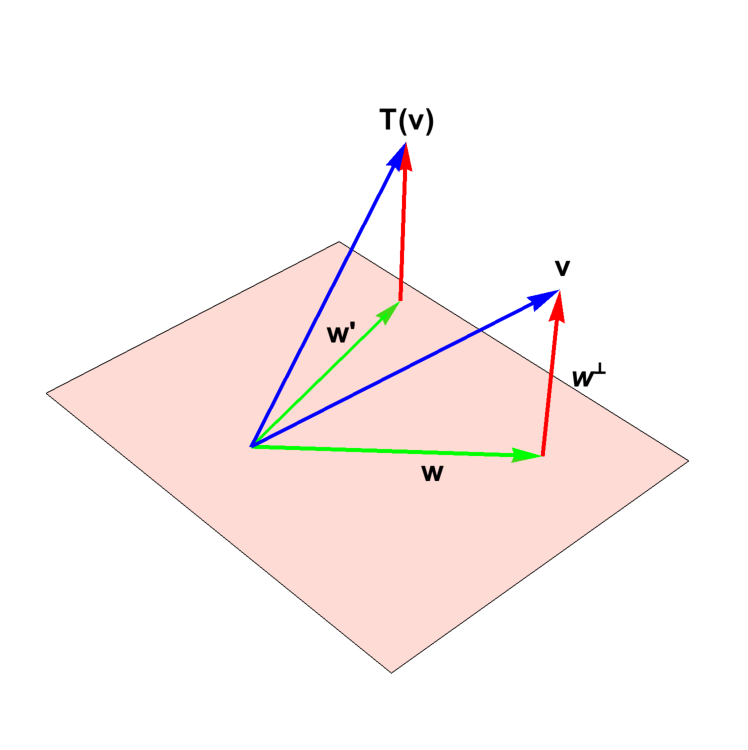
\includegraphics[width=2in]{GeneralRotation}
\]
Since rotation is an isometry that fixes the origin, $T$ is linear. As such we wish to come up with the matrix $A$ such that $T=T_A$. Below I outline two different methods. 
\\
(a) {\em Method 1}. Create a basis $B'$ of the form $\ds B'=\{ \boldw_1,\boldw_2,\boldn \}$, where $\boldw_1, \boldw_2$ are two orthonormal vectors in $W$. Compute $[T]_{B'}$ then convert everything to the standard basis $B$ using the change of basis formula for transformations. The basis $B'$ being orthonormal simplifies computations. 
\\  
(b) {\em Method 2}. (Requires the cross product) Given $\boldv=(x,y,z)$, describe $T(\boldv)$ in terms of the the three mutually orthogonal vectors  $\boldn$, $\boldw=\proj{\boldv}{W}$, and $\ds\boldw'=\boldn\times\proj{\boldv}{W}$. After some work you can derive the formula 
\[
T(\boldv)=\cos(\theta)\boldv+\sin(\theta)(\boldn\times\boldv)+((1-\cos \theta)\boldv\cdot\boldn)\boldn.
\]
Writing $\boldn=(a,b,c)$ and evaluating this formula for $T$ at $\boldv=(1,0,0), (0,1,0)$ and $(0,0,1)$ will give us the three columns of our matrix, expressed in terms of $a, b, c$ and $\theta$.  
\\
\begin{solution}
%\ \\
\noindent
I'll let you think about this one some more. 
\end{solution}
\ee
